\documentclass[12pt,a4paper,titlepage]{article}
\usepackage[left=2.5cm,text={16cm,20cm},top=4cm]{geometry}
\usepackage[T1]{fontenc}
\usepackage[czech]{babel}
\usepackage[utf8]{inputenc}
% dalsi balicky
\usepackage{graphicx}
\usepackage{enumitem}
\usepackage{indentfirst}
\usepackage{float}
\usepackage{svg}
\usepackage{amsmath}
\usepackage{url}
\usepackage{graphics}
\usepackage{graphicx}
\graphicspath{ {images/} }
\usepackage[bookmarksopen,colorlinks,plainpages=false,urlcolor=blue,
unicode,linkcolor=black]{hyperref}

\bibliographystyle{czplain}

%úvodzovky
\providecommand{\uv}[1]{\quotedblbase #1\textquotedblleft}

\begin{document}

\begin{titlepage}
\begin{center}
    {
    	\Huge\textsc{Vysoké učení technické v~Brně}}\\
    \smallskip
    {
    	\huge\textsc{Fakulta informačních technologií}}\\
    \bigskip
    \vspace{\stretch{0.382}} %pomery odpovedajúcí zlatému rezu    
    \huge{Modelování a simulace}\\
    \smallskip
    \Huge{Projekt - model supermarketu}\\
    \vspace{\stretch{0.618}}
\end{center}
    {\Large \today \hfill David Kozák (xkozak15)  }\\
    \smallskip
    {\Large \hfill Peter Miklánek (xmikla10)}
\end{titlepage}

\newpage
\tableofcontents
\newpage

\section{Úvod}
V této práci je řešena implementace modelu(viz \ref{prezentace} slide 7) obchodu s potravinami v rámci projektu do IMS.
Na základě modelu a simulačních experimentů bude ukázáno chování systému v nejvytíženějším obodobí dne. Smyslem experimentu je demonstrovat, že pokud by v běžně velkém supermarketu některé normální pokladny byly nahrazeny samoobslužnými, bude to mít pozitivní účinek na celý systém, konkrétně řečeno dojde ke snížení průměrných i maximálních front u pokladen a ke snížení průměrné doby strávené čekáním u pokladny.
\subsection{Autoři podílející se na práci a odborné konzultace}
Celou práci navrhli a implementovali studenti třetího ročníku bakalářského studia na FIT VUT v Brně David Kozák a Peter Miklánek. Práce byla konzultována s vedoucím prodejny, která byla modelována , a s jejími řadovými zaměstnanci. 
\subsection{Informace o simulovaném systému}
Pro naše experimenty jsme zvolili konkrétní supermarket Lidl ve Slatině na adrese Hviezdoslavova 1288/2. Do tohoto obchodu chodíme pravidelně nakupovat, proto jsme data pro modelování sbírali nevědomky již dlouho dobu dopředu. Obchod je dobře zařízený a většinu dne lze nákup vyřídit celkem rychle. Funguje tu až sedm pokladen, z nichž je většinou pouze několik aktivních, nicméně v intervalu mezi 16-19 hodin dochází tradičně k velkým frontám, protože lidé jezdí domů z práce a chtějí nakupovat. Čekání v těchto frontách může být velmi iritující. V rámci zlepšení situace  navrhujeme místo dvou současných pokladen zařídit 6 samoobslužných. Nejdříve tedy modelujeme současný stav obchodu a poté upravenou verzi se samoobslužnými pokladnami. Následně pomocí experimentů ověříme, zda tato změna má chtěný efekt na maximální a průměrnou délku front a snížení doby strávené ve frontě, čímž chceme dokázat, že tato změna by skutečně měla pozitivní vliv na zkušenost zákazníků.
\subsection{Ověřování validity modelu}
Validitu našeho modelu jsme ověřovali za pomoci naměřených dat a poznatků získaných pozorováním a měřením skutečného systému, tedy pobočky Lidlu. Veškeré výsledky získané při prvních simulacích byly porovnávány se skutečným systémem a v případně výrazných nesrovnalostí jsme náš abstraktní model několikrát upravovali, aby co nejlépe odpovídal realnému systému.
\section{Rozbor tématu a použitých metod/metodologií}
Vzhledem k relativně lehkému sbírání skutečných dat jsme model validovali vlastními měřeními a internetové zdroje jako například \ref{google-shop} jsme používali pro porovnání s výsledky našich měření. Po důkladné analýze jsme získali o systému následující informace. 

\subsection{Použité postupy pro vytváření modelu}
Pro vytváření abstraktního modelu byla využita Petriho síť, neboť umožňovala přehledně znázornit modelovaný systém. Pro vytváření simulačního modelu byla využita knihovna SIMLIB psaná v jazyce C++. Podrobné informace o využitých konstrukcích a algoritmech lze nalézt například v ......


Ve zvoleném období přichází zákazníci do obchodu v intervalech daných exponenciálním rozdělením se středem 18 vtěřin. Část zákazníků přijede autem a parkuje na parkoviště, část jich přijde pěšky či městskou hromadnou dopravou. Po příchodu do obchodu si zákazníci zaberou buď vozík nebo košík. Ve velice nepravděpodobném případě, že nejsou žádné vozíky ani košíky k dispozici, zákazníci 10 vteřin čekají a pokud žádný košík či vozík nezískají, odcházejí nakupovat do vedlejší prodejny. Velmi malá skupina zákazníků do Lidlu vejde pouze proto, aby provedla nákup v masně, který je uvnitř budovy, ale vně samotného obchodu. Pro příchod do obchodu musí zákazníci projít bránou, do které se vejde najednou maximálně jeden člověk. Tato akce zabere průměrně tři vteřiny. Poté probíhá samotný nákup, jehož délka je opět dána exponenciálním rozložením se středem 20 minut. Po dokončení nákupu odchází zákazníci k pokladnám a stoupnou si do nejkratší fronty. Až na ně přijde řada, vyloží svůj nákup na pokladní pás a proběhne interakce s pokladní, jejíž délka je dána exponenciálním rozložením se středem 90 sekund. V přibližně 3\% procentech případů při scanování nákupu dojde k chybě a musí být zavolána vedoucí prodejny, aby vzniklý problém vyřešila. Její příchod je dán exponenciálním rozložením se středem 3 minuty a vyřešení vzniklého problému trvá dobu danou exponenciálním rozložením se středem 1 minuta. Po dokončení nákupu ještě 20 \% lidí jde koupit maso do masny. Zde pracují dva prodavači a doba obsluhy jednoho zákazníka trvá dobu danou exponenciálním rozložením se středem 1 minuta. Pokud by zákazníci nebyli do tří minut obslouženi, z obchodu odchází. Po dokončení návštěvy masny již zákazníci vrátí svůj vozík či košík a následně odcházejí z obchodu. 5\% z nich si ale ještě při odchodu uvědomí, že na něco zapomněli, a proto se znovu do  obchodu vrací. Nijak je v modelu nerozlišujeme od normálních zákazníků vyjma fakt, že jejich nákup trvá výrazně kratší dobu danou exponenciálním rozložením se středem 3 minuty.

Dalšími důležitými osobami jsou zaměstanci prodejny. Těch je v obchodě stabilně 7-9 a jejich životní cyklus je následující. Zaměstanci mají na starost čtyři rozdílné činnosti, mezi kterými se rozhodují na základně priorit. Nejprioritnější činností je obsluha pekárny. Ta trvá dobu danou exponenciálním rozložením se středem 20 minut. Následně pekárna funguje po dobu 1 hodiny bez obsluhy, poté je potřeba ji znovu obsloužit. K pokladně se zaměstnanec přesune, pokud bude alespoň jedna pokladna uzavřena a průměrná délka front bude větší než 6 zákazníků. Zaměstanec pokladnu uzavírá, pokud je průměrná délka ve frontách kratší než 4 zákazníci. Pokud zaměstnanec nemusí jít k pekárně ani pokladnám, zbývají ještě dvě další činnosti. Zaměstnanec si může na dobu 30-ti minut vzít pauzu, nicméně na tuto pauzu má nárok pouze jednou v průběhu experimentu. Pokud není ani jedna z předchozích činností proveditelná, zaměstnanec bude po dobu 30-ti minut doplňovat zboží a poté znovu provede zhodnocení situace a případně půjde provést jinou činnost. Část zaměstnanců může pracovat pouze na skladě a celý den doplňovat zboží.

\section{Koncepce}
Cílem projektu je simulovat obchod v jeho nejvytíženějším období. Vzhledem k cíli práce je nutné vytvořit modely dva, první model pro současnou situaci a druhý model pro variantu se samoobslužnými pokladnami. 

\subsection{Modelářská témata}
\subsubsection{Abstrahování}
Vzhledem k faktu, že simulace se zaměřuje hlavně na údaje o frontách před pokladnami, je možné některé aspekty skutečného systému zanedbat. Při vytváření abstraktního modelu došlo k následujícím abstrakcím. 
\begin{itemize}
\item Jednotlivé osoby, pokud přijdou ve skupině a nakupují spolu, jsou modelovány jako jeden proces zákazníka.
\item Osoby, které si pouze koupí maso v masně a poté opět odejdou, nejsou v systému modelovány vůbec, protože nepřijdou vůbec do styku s pokladnami, jejichž vlastnosti tato práce zkoumá. 
\item Problém parkoviště a parkovacích míst je též zanedbaný, neboť při měřeních bylo zjištěno, že k jeho zaplnění nedochází.
\item Pracovníci, kteří jsou pouze na skladě či doplňují zboží, jsou též zanedbání, neboť jejich činnost neovlivňuje situaci u pokladen. 
\item V případě modelu se samoobslužnými pokladnami je jeden zaměstnanec přidělen k těmto pokladnám na celý den, je tudíž modelován pouze jako obslužná linka pro případné dotazy či asistenci.
\item Košíky a vozíky jsou abstrahovány jako jedno skladiště, neboť pro účely této práce není nutné tyto dva předměty rozlišovat.   
\end{itemize}


\subsubsection{Formální popis abstraktního modelu}
Jako formalismus pro zápis abstraktního modelu byla zvolena Petriho síť, kterou můžete vidět na následujícím obrázku. Barvy přechodů a stavů jsou použity pouze pro zvýšení přehlednosti obrázku a také pro legendu. Jako formální definice je využita ODKAZ  \\

\begin{figure}[h]
\centering
\includegraphics[scale=0.3]{supermarketadvanced}
\caption{Petriho síť modelující supermarket}
\end{figure}


Výše uvedený model již zahrnuje i samoobslužné pokladny. Z toho tedy vyplývá, že se už jedná o rozšířený model. Verzi modelující současný stav můžete najít v příloze . Do jádra dokumentu nebyla vložena, neboť se od rozšířeného modelu téměř neliší, jediný rozdíl tkví v absenci části modelu, která reprezentuje samoobslužné pokladny. 

Některé pokročilé podmínky by se v petriho síti špatně vyjadřovaly, proto jsou pouze znázorněny v legendě a poté zahrnuty až do simulačního modelu. Mezi takovéto podmínky patří například otevírací a uzavírací podmínka u pokladen.

\subsection{Implementační témata}
Program se skládá ze dvou modelů basic\_model a abstract\_model. Basic model modeluje současnou situaci v obchodu, zatímco abstract\_model již zahrnuje i samoobslužné pokladny. Při spuštění oba modely produkují relativně velké množství údajů, z nichž z hlediska této práce patří mezi nejzajímavější statistiky o využití pokladen, klasických i samoobslužných, a též histogram zobrazující průměrnou dobu strávenou čekáním před pokladnami. Detailnější popis implementace je uveden v následující kapitole. 

\section{Architektura simulačního modelu/simulátoru}
V této sekci jsou popsány implementační detaily obou modelů basic i advanced. Nejdříve jsou diskutovány rozšíření nad knihovnou SIMLIB umožňující jednodušší tvorbu samotného simulačního modelu. V další části jsou popsány důležité a zajímavé vlastnosti samotného simulačního modelu.
\subsection{Rozšíření tříd Process a Facility}
Jelikož abstrakce Process a Facility neposkytovaly všechny operace, které byly pro jednoduchou tvorbu simulačního modelu vhodné, autoři dané třídy rozšiřili. Výstupem operace rozšiřování jsou následující třídy. 

\begin{itemize}
\item TimeoutableProcess  - Jednoduché rozšíření třídy process přidávající metody pro práce s mechanismem timeout.
\item ClosableFacility -  Rozšíření třídy Facility, nad kterou je definována operace uzavření, otevření a zjištění stavu. Pokud nějaký proces nad takovouto Facility bude volat metodu Seize, dojde ke generování výjimky FacilityNotOpenedException. Tato abstrakce je užitečná v případech, kdy je potřeba modelovat zařízení, které může být v průběhu simulace otevíráno a uzavíráno. K uzavření nastane buď při explicitním zavolání metody close. 
\item MaintainableClosableFacility - Rožšíření třídy ClosableFacility, pro jehož obsluhu je potřeba vymezit proces, který se o jeho provoz stará. Pro otevření takovéto Facility je potřeba vyhradit proces, který bude po volání operace open pasivován až do doby, než bude facility znovu uzavřena. K tomuto dojde v případě, kdy jiný process nad Facility zavolá operaci close či při splnění podmínky ClosableFacilityClosingCondition, která je předávána objektu v konstruktoru a je interně testována v každé operaci Release. Při jejím splnění dojde k přechodu zařízení do stavu shutting down, ve kterém již není novým procesům umožněno vstoupit do fronty, ale procesy, které jsou již ve frontě přítomny, jsou obslouženy. Po obsloužení posledního z těchto procesů se Facility uzavírá a obsluhující proces je aktivován. 
\end{itemize}

\subsection{Popis simulačního modelu}
V simulačním modelu obchodu se vyskytují dva procesy. Prvním procesem je proces zákazníka, který do obchodu přichází, prování nákup, poté je obsloužen u pokladny, případně i u masny, a následně ze systému odchází. Zákazník je modelovaný pomocí třídy TimeoutableProces, neboť při čekání na vozík či košík a při čekání ve frontě u masny je definován časový limit, po jehož uplynutí odchází neobsloužen.

Druhým modelovaným procesem je zaměstanec. Vzhledem k popisu jeho činnosti popsány výše se může nacházet v jednom za čtyř stavů. Zaměstnanec buď obsluhuje pekárnu nebo obsluhuje zákazníky u pokladny nebo pracuje na skladě nebo má pauzu. Na počátku běhu simulace a následně po skončení právě prováděné činnosti si zaměstnanec na základě prioritního systému zvolí novou činnost. Nejprioritnější činností je starost o pekárnu. Vzhledem k faktu, že k nutnosti obsluhy pekárny dochází s hodinovými mezerami, není tato činnost příliš častá. Nejběžnější činností zaměstnance je obsluha zákazníků u pokladny. Další činnosti zaměstnance je doplňování zboží a pauza. V basic modelu je zaměstnanců 7, každý pro jednu pokladnu. V advanced modelu je zaměstanců pouze 5. Šestý zaměstnanec má na starosti samobslužné pokladny a je modelován pouze jako oblužná linka. Sedmý zaměstnanec není v modelu již potřeba. 

Pokladny jsou modelovány pomocí třídy MaintainableClosableFacility. K jejich obsluze je totiž nutná přitomnost zamětstnance, který v danou chvíli nemůže dělat žádnou jinou činnost. Podmínka ClosableFacilityCondition byla již zmíněna dříve a v tomto konkrétním případě nabývá hodnoty true pokud je průměrná délka u pokladen menší než 4. Zaměstanec je při vstupu do pokladny pasivován a následně znovu aktivován po jejím uzavření, ke kterému dojde při splnění podmínky pro uzavření, přechodu do stavu shutting down a následnému vyprázdnění fronty. 

Masna je modelována jako Skladiště s velikostí 2, ke kterému přichází pouze 20 \%  procesů. Tyto procesy, jak již bylo zmíněno výše, z fronty odcházejí, pokud jejich obsluha nezapočne dříve než za 3 minuty od počátku čekání ve frontě. 

Pekárna je modelována speciálním způsobem. Je reprezentována pouze jednou proměnnou Boolovského typu, k jejímu označení se dále bude používat výraz flag. Pokud zaměstanec zjistí, že daný flag má hodnotu true, začne obsluhovat pekárnu.  Prvním krokem této obsluhy je  nastavení flagu do hodnoty false. Dále je proces zaměstance pasivován funkcí Wait na dobu danou exponenciálním rozložením se středem 20 minut. Jakmile je zaměstnanec opět aktivován, naplánuje Event v čase Time + 1 hodina, který hodnotu flagu opět nastaví do hodnoty true. 

Vozíky a košíky jsou modelovány jako jedno skladiště s kapacitou 300. 

Speciální částí advanced modelu jsou samoobslužné pokladny. K nim přichází pouze určité procento zákazníků a to pouze tehdy, pokud je celková fronta tvořená před nimi kratší než 10 zákazníků. Jedná se o skladiště s kapacitou 6. Jelikož při samobslužných pokladnách lidé často chybují, s 10\%  pravděpodobností budou zákazníci potřebovat poradit, k čemuž je vyhrazena obslužná linka modelující zaměstance, který má samoobslužné pokladny na starost.  


\section{Podstata simulačních experimentů a jejich průběh}
Cílem této práce je dokázat, že instalace šesti samoobslužných pokladen za cenu ztráty dvou normálních bude mít pozitivní účinek na dobu strávenou ve frontách i na průměrnou a maximální délku front. Pro experimentování bylo ale nejdříve potřeba najít nejvhodnější všech vstupních údajů tak, aby výsledný model co nejvěrohodněji modeloval skutečný systém. 

\subsection{Postup experimentování}
První fází byla validace modelu. Jejím výstupem byl abstraktní model, který z pohledu autorů v dostatečné míře modeloval původní systém obchodu. Dalším krokem byla tvorba simulačního modelu. První experimenty s ním sloužili hlavně za účelem verifikace modelu. Tento proces obnášel porovnávání výsledků běhů simulace s naměřenými daty. Nutno podotkonout, že v této fázi několikrát došlo k úpravám abstraktního modelu, protože se zjistilo, že nebyl dostatečně validní. 

Jakmile autoři dospěli do bodu, kdy dle jejich uvážení základní simulačního model dostatečně přesně modeloval skutečný systém, byla zahájena tvorba pokročilého simulačního modelu, který již zahrnoval výše zmíněné samoobslužné pokladny. Zde byla problematika validace a verifikace náročnější, neboť skutečná data z pochopitelných důvodů nemohla být naměřena. Tento model totiž modeluje verzi obchodu, která zatím neexistuje. Autoři tedy byli nuceni výsledky validovat pouze na základě svého vlastního odhadu a za pomoci dat z jiných prodejen, které již mají samoobslužné pokladny zavedené.

\subsection{První experimenty}
První experimenty byly spouštěny za účelem ověřování validity modelu. Nenaštěstí bylo zjištěno, že vytvořený model přiliš realitě neodpovídal. Tvořily se v něm příliš dlouhé fronty, průměrná doba strávená na pokladnách dosahovala až jedné hodiny, což bylo nepřijatelné. Výstup můžete vidět na níže uvedeném histogramu. 

\begin{figure}[h]
\centering
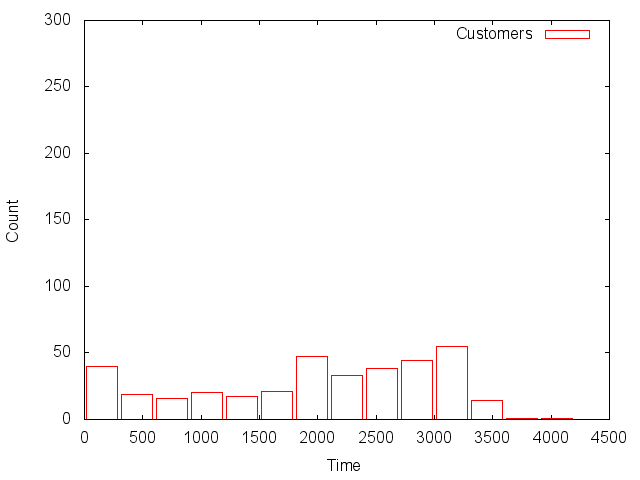
\includegraphics[scale=0.75]{awful}
\caption{Histogram doby strávenené čekáním u pokladen v nevalidním modelu}
\end{figure}

Fronty navíc způsobovaly vyprázdnění skladiště na vozíky a velký počet zákazníků, kteří ze systému odešli po deseti vteřinách bez vozíků. Aby došlo k odstranění tohoto jevu, bylo zapotřebí provést následující úpravy:
\begin{itemize}
\item změna střední hodnoty exponenciálního rozdělení příchodu zákazníků z 11 vteřin na 18 vteřin
\item snížení výskytu chyb u zaměstanců na pokladně z 5 \% na 3 \%
\item zvýšení doby timeoutu masny na 3 minuty
Po výše uvedených úpravách již výstupy modelu dostatečně odpovídaly skutečnému systému. 
\end{itemize}
\subsection{Experimenty se základním modelem}
Výsledky je možné vidět na následujícím histogramu. Pro účely ověření je tento experiment možno spustit příkazem ./basic .

\begin{figure}[h]
\centering
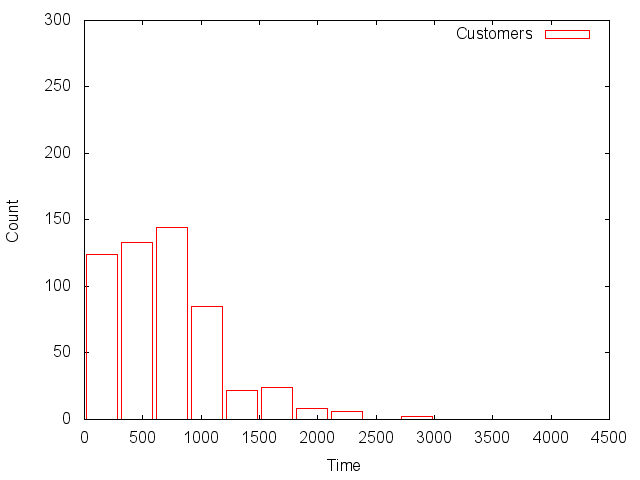
\includegraphics[scale=0.75]{basic}
\caption{Histogram doby strávené čekáním u pokladen v základním modelu}
\end{figure}

\subsection{Experimenty s rozšířeným modelem}
Tyto experimenty sloužily k získání představy o tom, jakým způsobem bude systém ovliněn při výše zmíněné výměně dvou normálních pokladen za šest samoobslužných. Výsledky je možné vidět na následujícím histogramu. Výsledky je možné vidět na následujícím histogramu. Pro účely ověření je tento experiment možno spustit příkazem ./advanced .

\begin{figure}[h]
\centering
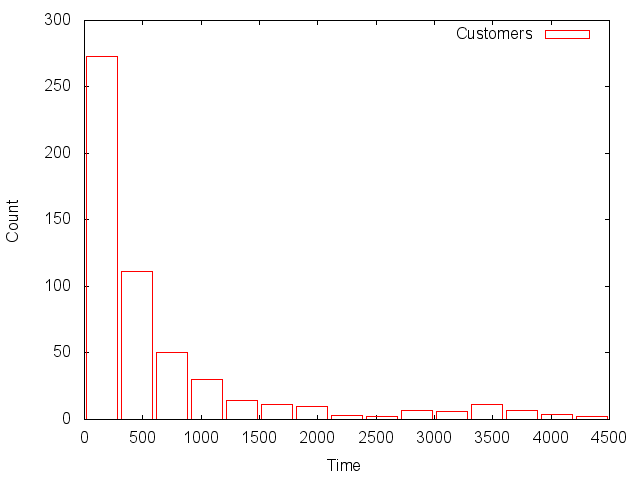
\includegraphics[scale=0.75]{advanced}
\caption{Histogram doby strávené čekáním u pokladen v rozšířeném modelu}
\end{figure}

\subsection{Srovnání experimentů}
Ze srovnání histogramů dvou předchozích experimentů je patrné, že průměrná doba strávená skutečně poklesla. Tento pokles je dokonce poměrně výrazný a dle názoru autorů by ho jistě zákazníci uvítali. Jako zajímavé zjištění může být uveden fakt, že navzdory počátečním úvahám bylo při experimentech zjištěno, že budou bohatě stačit tři samoobslužné pokladny, neboť průměrné využití skladiště, které je modelovalo, málokdy dosáhlo vyšších hodnot průměrného využití než 3. 
\subsection{Popis použití simulátoru}





\section{Shrnutí simulačních experimentů a závěr}
V tomto projektu byl modelován supermarket Lidl na adrese Hviezdoslavova 1288. Validita modelu byla ověřena daty získanými při měření. Cílem experimentů bylo prokázat, že instalace šesti samoobslužných pokladen za cenu odstranění dvou normálních bude mít pozitivní účinek na délku fronty. Na základě experimentů bylo zjištěno, že po nainstalování samobslužných pokladen skutečně dojde ke snížení doby čekání ve frontách i ke snížení průměrných délek front u pokladen. Také bylo zjištěno, že navdory původní předpokladům, pro dosažení cíleného účinku budou stačit pouze tři samoobslužné pokladny místo původních šesti. V rámci projektu též vznikla nová abstrakce nad knihovnou SIMLIB. Toto rozšíření   obsahuje třídy TimeoutableProcess,ClosableFacility a MaintainableClosableFacility. 


V této části popíšeme data získaná z oficiálních zdrojů lidlu a také je srovnáme s naším vlastním měřením.
\subsection{Meření}
\subsection{První měření 21.11.2016 17:30}
V průběhu 5-ti minut přišlo do obchodu 32 lidí.

Parkoviště je hodně velké, ještě jsem neviděl, že by se zaplnilo, asi toto můžeme ignorovat, z pohledu pokladen není podstatné.
Na parkovišti parkovišti je k dispozici 150+ vozíků, nevidím realně, že by došly.
\\
Je tam masna se dvěma prodavači a trafika s jednou prodavačkou.

V obchodě je 7 pokladen, jelo jich 5. Jednou za čas potřebují pokladny pomoci od vedoucí vyřešit problém.

Je tam pekárna, jednou za čas do ní někdo ze zaměstnanců odběhne a má tam sex.

Můj nákup trval sedm minut bez pokladny. Petrův nákup trval také sedm minut.

\subsection{Doba u pokladny}
Naměřeno u jedné pokladny než ji zavřeli.
\begin{itemize}
\item 1:05
\item 1:37
\item 0:40
\item 1:47
\item 1:06
\end{itemize}
Naměřeno Petrem
\begin{itemize}
\item 03:04
\item 00:42
\item 01:23
\item 03:47
\item 02:14
\end{itemize}


\textbf{Bylo by dobré naměřit více dat :) }


\begin{center}
    \begin{tabular}{| l | l | }
    \hline
    Jméno  třídy & Popis třídy  \\ \hline
    TimeoutableProcess & Jednoduché rozšíření třídy process přidávající metody pro práce s mechanismem timeout. \\ \hline
    ClosableFacility &  Rozšíření třídy Facility, které je možné uzavřít. \\ \hline
    MaintainableClosableFacility & Rožšíření třídy ClosableFacility, pro jehož obsluhu je potřeba vymezit proces, který se o jeho provoz stará.  \\
    \hline
    \end{tabular}
\end{center}

\section{Závěr}
\begin{enumerate}[label={[\arabic*]}]
\item PERINGER P. Slajdy k přednáškám modelování a simulace, 2016. Verze  2016-09-20 [cit. 2016-12-05][Online] \\
     \href{https://www.fit.vutbr.cz/study/courses/IMS/public/prednasky/IMS.pdf}
          {https://www.fit.vutbr.cz/study/courses/IMS/public/prednasky/IMS.pdf}
     \label{prezentace}

\item PERINGER P. SIMulation LIBrary for C++, 2011. [Online] \\
    \href{https://www.fit.vutbr.cz/~peringer/SIMLIB/}
         {https://www.fit.vutbr.cz/~peringer/SIMLIB/}
    \label{demo1}

\item HRUBÝ M. Demonstrační cvičení IMS \#1, [cit. 2016-12-05][Online] \\
    \href{http://perchta.fit.vutbr.cz:8000/vyuka-ims/uploads/1/ims-demo1.pdf}
        {http://perchta.fit.vutbr.cz:8000/vyuka-ims/uploads/1/ims-demo1.pdf}
    \label{demo2}

\item HRUBÝ M. IMS democvičení \#2, [cit. 2016-12-05][Online] \\
    \href{http://perchta.fit.vutbr.cz:8000/vyuka-ims/uploads/1/diskr2-2011.pdf}
        {http://perchta.fit.vutbr.cz:8000/vyuka-ims/uploads/1/diskr2-2011.pdf}
    \label{simlib}

\item Statistické informace Googlu o modelované prodejně \\
     \href{http://goo.gl/6zOMvi}
          {http://goo.gl/6zOMvi}
     \label{google-shop}
\end{enumerate}
\end{document}